\subsection{Connecting to the application and getting the source code}
This section will explain how to get the FeedJam source code and how you can visit a running version of the application on our own server.

The application's source code is hosted as an open repository on the web service GitHub.com. This means that you have several different ways of downloading our source code. Our repository is available from \url{https://github.com/lha047/IrProject}. From this url you can either download the whole repository from within your browser, or you can fork/clone it from within your prefered Git utility. The reposityory has two branches, the one you will want to download is the "main" branch.

FeedJam is also running on \url{http://feedjam.thunemedia.no}, where you can test the whole application without setting it up locally on your own computers. Please keep in mind that you will run out of Twitter requests quite quickly due to the fact that we have been unable to cache a large enough portion of the Twitter user base. If you run out of requests but wish to continue testing the application you will need a new IP-adress (which you can get through for instance re-connecting to the UiB VPN). Note that we cannot promise that the web server is running at all times since we will not have physical access or control over it during the summer. 

\subsection{Screenshots}
\begin{figure}[ht]
    \begin{minipage}[b]{1\linewidth}
        \centering
        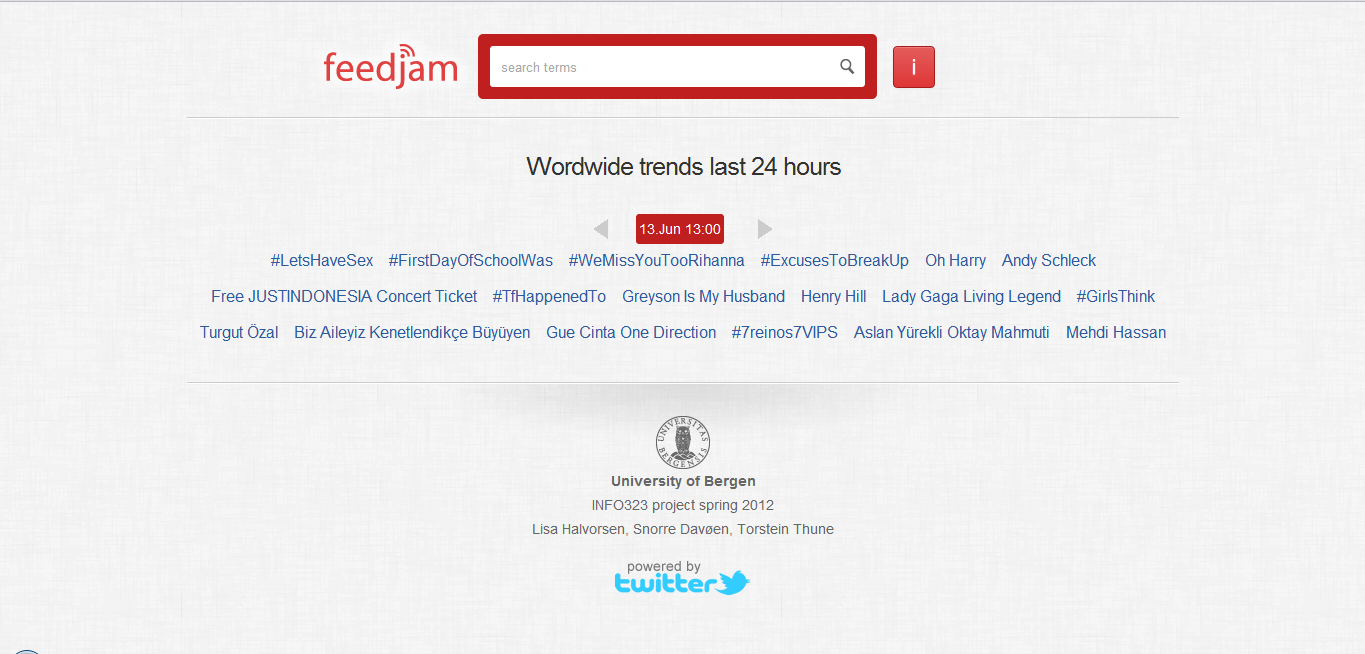
\includegraphics[width=1\textwidth]{figures/feedjam_frontpage_screenshot}
        \caption{The FeedJam frontpage}
        \label{fig:feedjamfrontpage}
    \end{minipage}
\end{figure}

\begin{figure}[ht]
    \begin{minipage}[b]{1\linewidth}
        \centering
        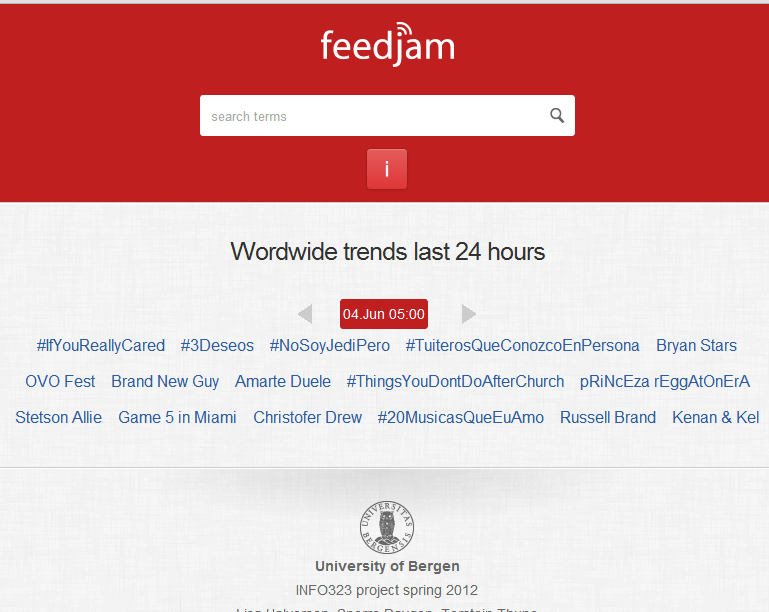
\includegraphics[width=1\textwidth]{figures/feedjam_responsive_frontpage}
        \caption{The FeedJam frontpage on lower resolutions}
        \label{fig:feedjamfrontpageresponsive}
    \end{minipage}
\end{figure}

\begin{figure}[ht]
    \begin{minipage}[b]{1\linewidth}
        \centering
        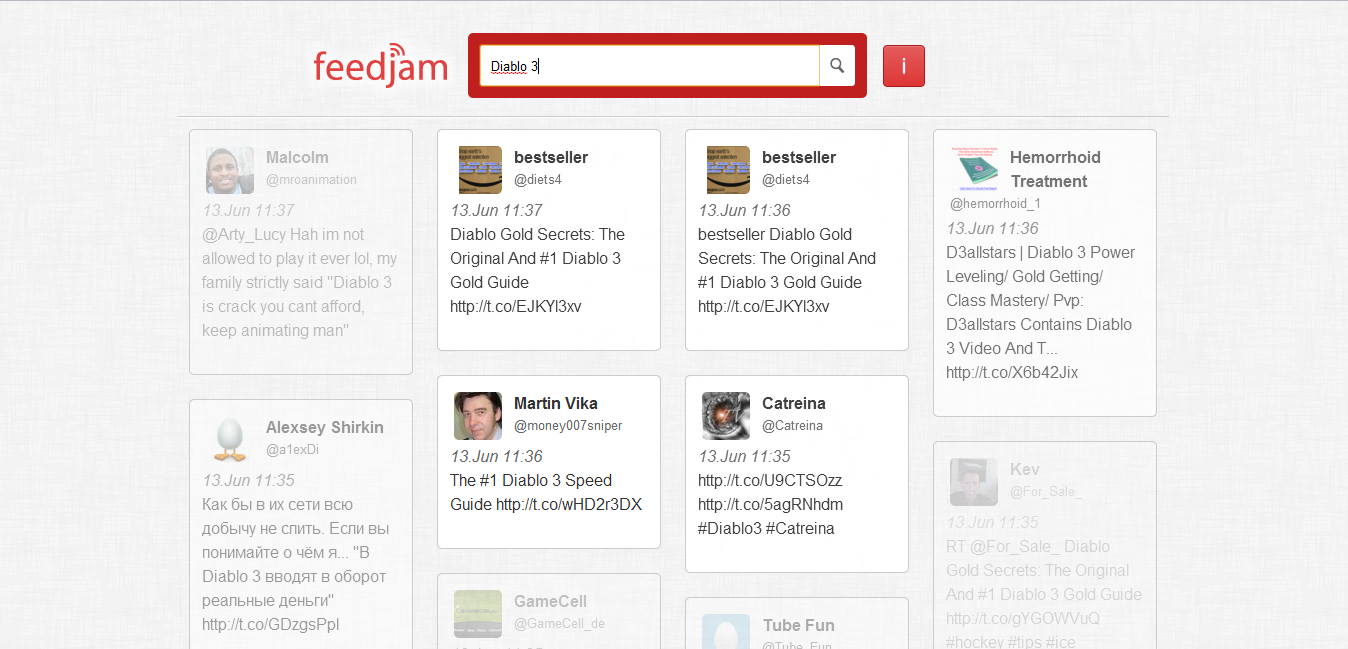
\includegraphics[width=1\textwidth]{figures/feedjam_search_screenshot}
        \caption{Search results}
        \label{fig:feedjamsearchresults}
    \end{minipage}
\end{figure}

\begin{figure}[ht]
    \begin{minipage}[b]{1\linewidth}
        \centering
        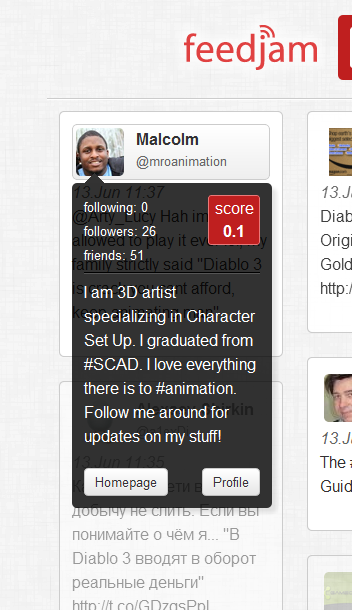
\includegraphics[width=0.7\textwidth]{figures/feedjam_user_screenshot}
        \caption{Displaying user information}
        \label{fig:feedjamuseropened}
    \end{minipage}
\end{figure}

\begin{figure}[ht]
    \begin{minipage}[b]{1\linewidth}
        \centering
        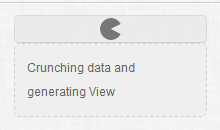
\includegraphics[width=1\textwidth]{figures/feedjam_loading}
        \caption{The FeedJam loading bar}
        \label{fig:feedjamloading}
    \end{minipage}
\end{figure}

\begin{figure}[ht]
    \begin{minipage}[b]{1\linewidth}
        \centering
        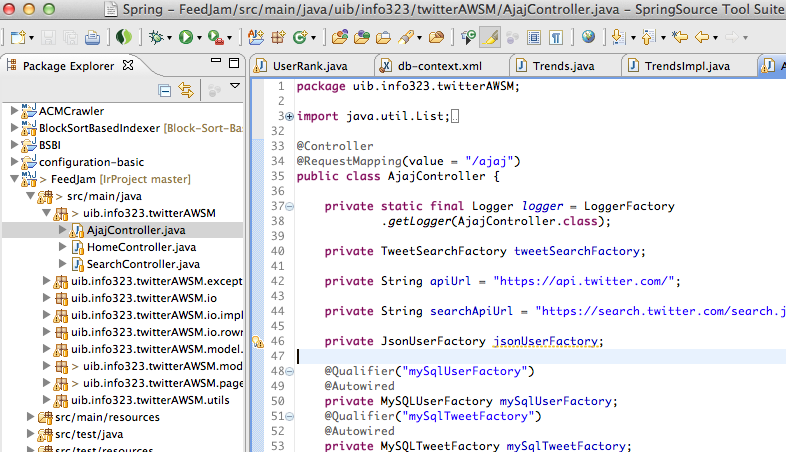
\includegraphics[width=1\textwidth]{figures/springsourcetoolsuite}
        \caption{The SpringSource Tool Suite IDE}
        \label{fig:springsourcetoolsuite}
    \end{minipage}
\end{figure}

\begin{figure}[ht]
    \begin{minipage}[b]{1\linewidth}
        \centering
        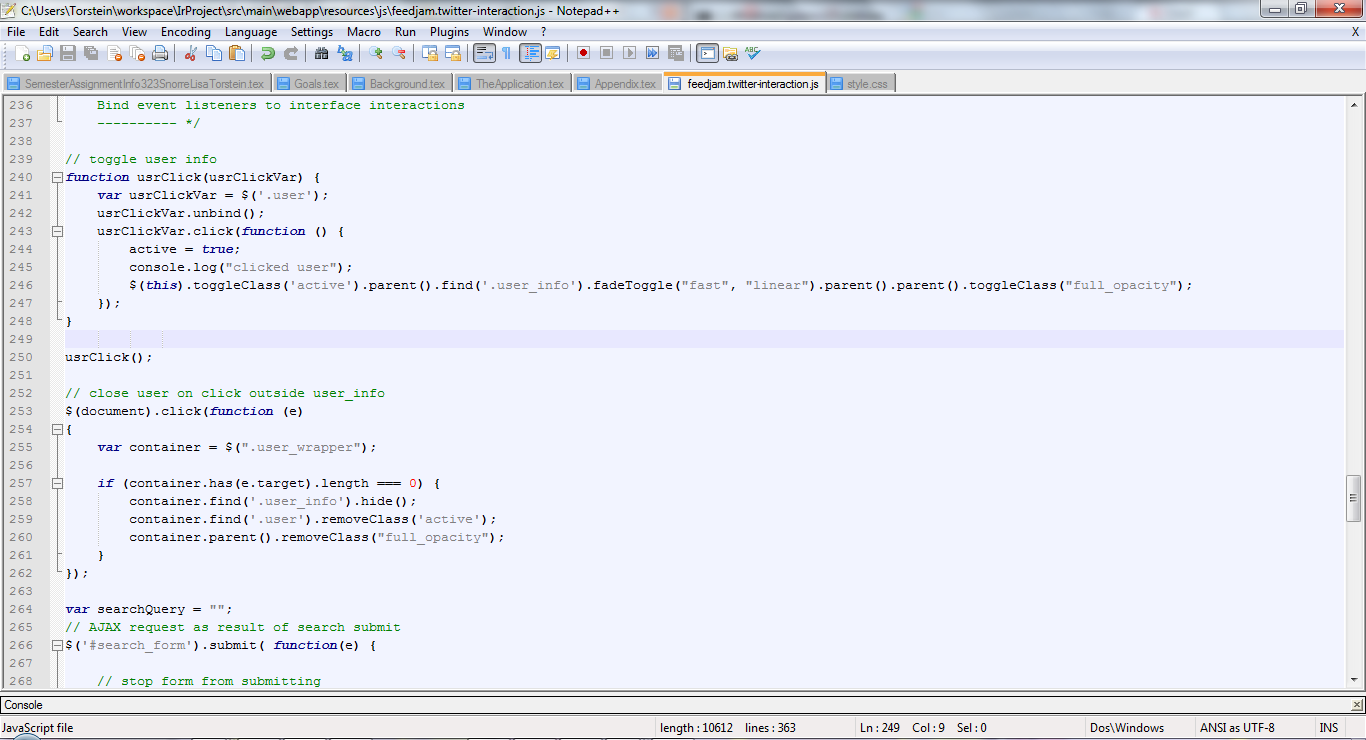
\includegraphics[width=1\textwidth]{figures/notepadplusplus}
        \caption{The Notepad++ text editor}
        \label{fig:notepadplusplus}
    \end{minipage}
\end{figure}

\begin{figure}[ht]
    \begin{minipage}[b]{1\linewidth}
        \centering
        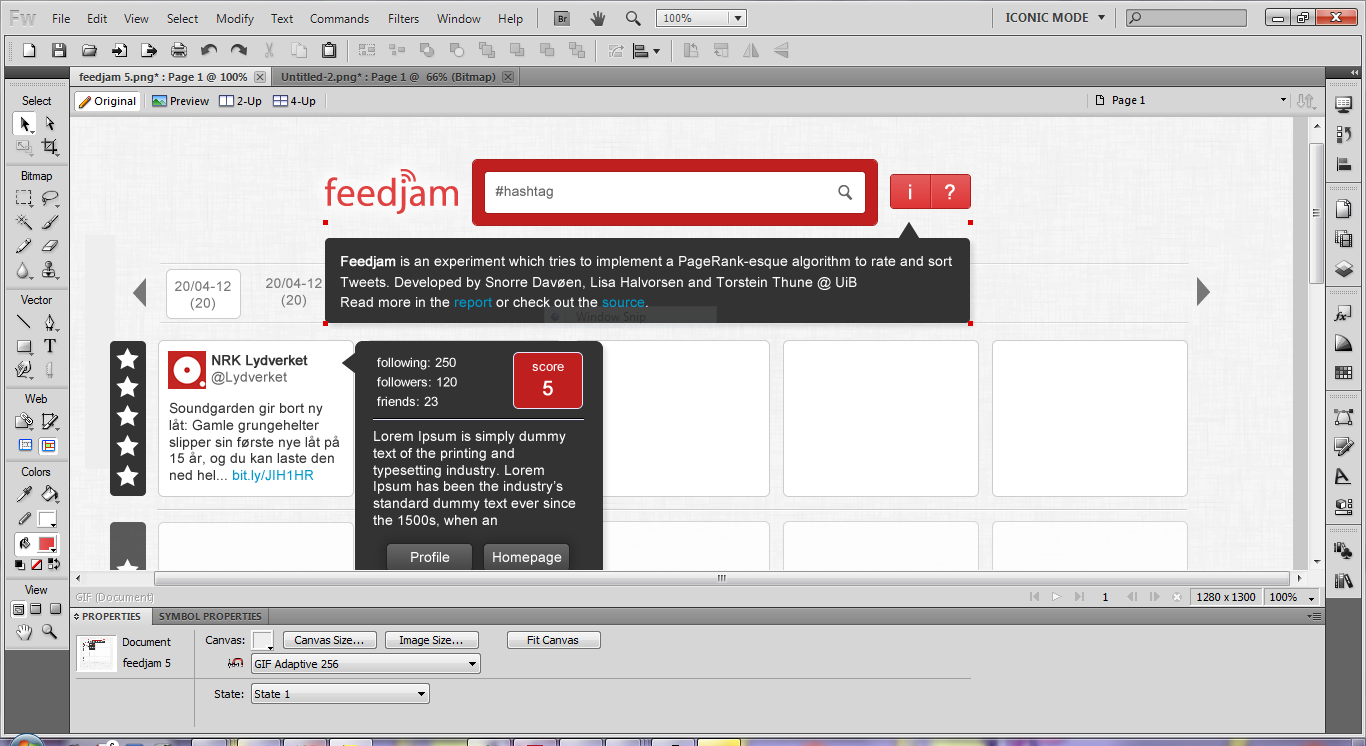
\includegraphics[width=1\textwidth]{figures/fireworks}
        \caption{Adobe Fireworks, a design/mockup utility}
        \label{fig:fireworks}
    \end{minipage}
\end{figure}